% Euclidean Handout Number Ten
\documentclass{tufte-handout}

%\geometry{showframe}% for debugging purposes -- displays the margins

%%%% Packages to make things pretty
\usepackage{amsmath,amsthm}
\usepackage{booktabs}
\usepackage{graphicx}
\setkeys{Gin}{width=\linewidth,totalheight=\textheight,keepaspectratio}
\graphicspath{{graphics/}}
\usepackage{units}
\usepackage{fancyvrb}
\fvset{fontsize=\normalsize}
\usepackage{multicol}
\usepackage{pdfpages}
\usepackage{fourier}

%%%% Theorem Environments
\theoremstyle{definition}
\swapnumbers
\newtheorem{problem}{Problem}[section]
\newtheorem{conjecture}[problem]{Conjecture}
\newtheorem*{definition}{Definition}
\newtheorem*{theorem}{Theorem}
\newtheorem{question}[problem]{Question}
\newtheorem{challenge}[problem]{Challenge}
\newtheorem*{postulate}{Postulate}

%%%%%

\title{Euclidean Geometry:\\An Introduction to Mathematical Work}
\author[]{Math 3600}
\date{Spring 2021}

\begin{document}

\maketitle

\begin{marginfigure}
    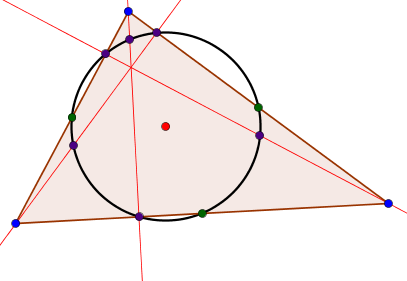
\includegraphics{NPC}
\end{marginfigure}

\setcounter{section}{10}
\section{Circles, Coming 'Round Again}
One of the most useful results about circles is Proposition III.20 which relates an \emph{inscribed} angle in a circle to a \emph{central} angle in that circle.
Let us try to see what happens when the angle does not sit on the circumference of the circle.

\begin{conjecture}
Let $\Gamma$ be a circle with center $O$. Let $X$ be a point in the interior of the circle, and suppose that two lines $\ell$ and $m$ intersect at $X$ so that $\ell$ meets $\Gamma$ at points $A$ and $A'$ and $m$ meets $\Gamma$ at $B$ and $B'$.
Then twice angle $AXB$ is congruent to angle $AOB$ and angle $A'OB'$ taken together.
\end{conjecture}

\begin{question}
Consider the situation from the last conjecture, but instead assume that $X$ lies outside $\Gamma$. What happens here? Formulate a conjecture.
\end{question}


\begin{conjecture}
If two chords of a circle subtend different acute angles at points of a circle, then the smaller angle belongs to the shorter chord.
\end{conjecture}

\begin{conjecture}
If a triangle has two different angles, then the smaller angle has the longer angle bisector (measured from the vertex to the opposite side).
\end{conjecture}

\begin{conjecture}[Steiner-Lehmus]
If a triangle has two angle bisectors which are congruent (measured from the vertex to the opposite side), then the triangle is isosceles.
\end{conjecture}

\begin{conjecture}
Let $BC$ be a chord of circle $\mathcal{C}$, let $\widearc{BC}$ be the arc of $\mathcal{C}$ which is bounded by $B$ and $C$ and does not contain the center of $\mathcal{C}$.
Let $M$ be the midpoint of $\widearc{BC}$.
For a point $A$ on the arc $\widearc{BC}$, show that as $A$ moves along the arc from $B$ to $M$, the sums $AB+AC$ increase.
\end{conjecture}


The next theorem is very pretty, and is commonly attributed to Archimedes.

\begin{conjecture}[Archimedes' Theorem of the Broken Chord] Let $AB$ and $BC$ be two chords of a circle $\mathcal{C}$, where $BC$ is greater than $AB$.
(Such a configuration is sometimes called a ``broken chord.'')
Let $M$ be the midpoint of arc ${ABC}$ and $F$ the foot of the perpendicular from $M$ to chord $BC$.
Then $F$ is the midpoint of the broken chord, that is, $AB$ and $BF$ taken together are congruent to $FC$.
\end{conjecture}

\vfill
\end{document}

%sagemathcloud={"zoom_width":100}